\section{実験装置}
図\ref{fig:実験装置}に変位センサとレバー系からなる実験装置の概略を示す.校正しようとする2本の変位センサはそれぞれ一軸ステージ1,2に載せられる.ステージを動かすことによって,変位センサのレバーに対する位置が調整できる.またレバーはマイクロメータヘッド3によって駆動される.なお,それぞれのステージやマイクロメータヘッドは手動で操作した.
\begin{figure}[htbp]
    \centering %中央揃え
    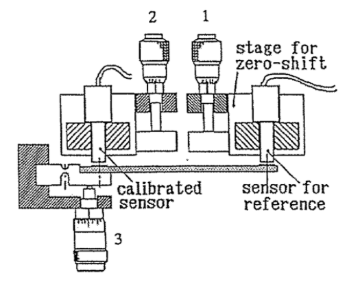
\includegraphics[width=100truemm,clip]{fig/fig_実験装置.png}
    \caption{Schematic diagram of experimental apparatus.}
    \label{fig:実験装置}
\end{figure}